\chapter{Architecture Overview}

\section{System Architecture}

The Chat Voting Chaos Chess Platform follows a modern, scalable architecture pattern optimized for serverless deployment on Vercel. The system is designed as a monorepo containing both frontend and backend applications.

\subsection{High-Level Architecture}

The platform consists of three main layers:

\begin{enumerate}
    \item \textbf{Presentation Layer}: Next.js frontend application
    \item \textbf{Application Layer}: Nest.js backend API
    \item \textbf{Data Layer}: PostgreSQL database with Prisma ORM
\end{enumerate}

\subsection{Architecture Diagram}

\begin{figure}[H]
    \centering
    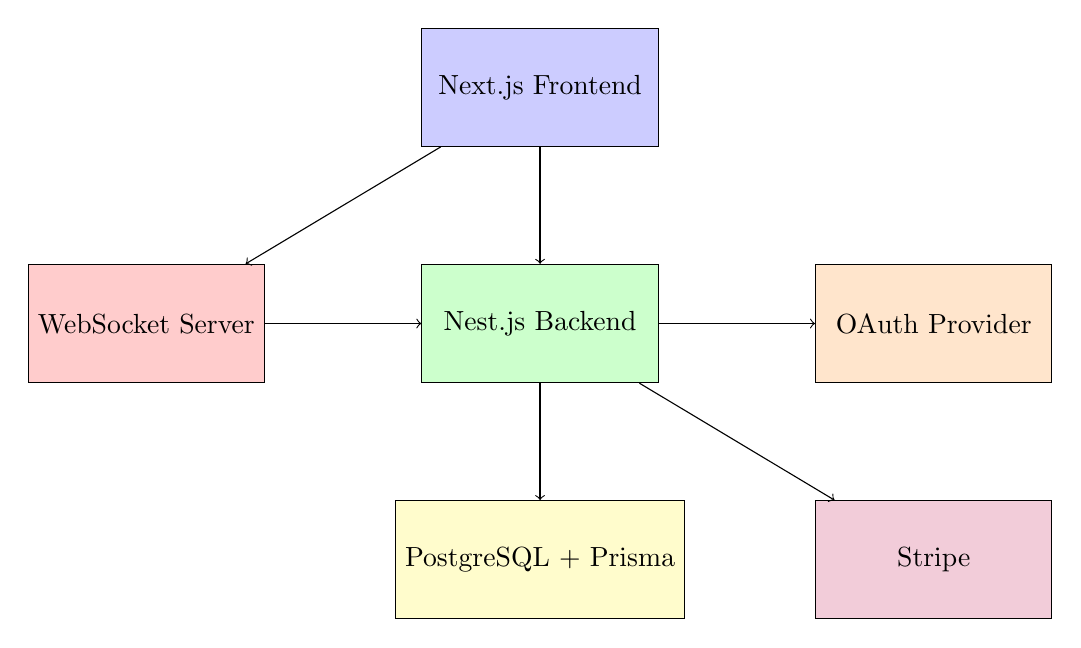
\begin{tikzpicture}[node distance=2cm]
        % Frontend
        \node[rectangle, draw, fill=blue!20, minimum width=3cm, minimum height=1.5cm] (frontend) {Next.js Frontend};
        
        % Backend
        \node[rectangle, draw, fill=green!20, minimum width=3cm, minimum height=1.5cm, below of=frontend, yshift=-1cm] (backend) {Nest.js Backend};
        
        % Database
        \node[rectangle, draw, fill=yellow!20, minimum width=3cm, minimum height=1.5cm, below of=backend, yshift=-1cm] (database) {PostgreSQL + Prisma};
        
        % External Services
        \node[rectangle, draw, fill=orange!20, minimum width=3cm, minimum height=1.5cm, right of=backend, xshift=3cm] (oauth) {OAuth Provider};
        \node[rectangle, draw, fill=purple!20, minimum width=3cm, minimum height=1.5cm, right of=database, xshift=3cm] (stripe) {Stripe};
        
        % WebSocket
        \node[rectangle, draw, fill=red!20, minimum width=3cm, minimum height=1.5cm, left of=backend, xshift=-3cm] (ws) {WebSocket Server};
        
        % Connections
        \draw[->] (frontend) -- (backend);
        \draw[->] (backend) -- (database);
        \draw[->] (frontend) -- (ws);
        \draw[->] (backend) -- (oauth);
        \draw[->] (backend) -- (stripe);
        \draw[->] (ws) -- (backend);
    \end{tikzpicture}
    \caption{High-Level System Architecture}
    \label{fig:architecture}
\end{figure}

\section{Monorepo Structure}

The project follows a monorepo pattern with the following structure:

\begin{lstlisting}[language=bash, caption=Monorepo Directory Structure]
chat-voting-chaos-chess/
├── apps/
│   ├── frontend/          # Next.js application
│   └── backend/           # Nest.js application
├── packages/
│   ├── shared/            # Shared TypeScript types and utilities
│   ├── prisma/            # Prisma schema and migrations
│   └── ui/                # Shared UI components
├── spec/                  # This specification document
└── package.json           # Root package.json for workspace
\end{lstlisting}

\section{Design Patterns}

\subsection{Backend Patterns}

The Nest.js backend implements several design patterns:

\begin{itemize}
    \item \textbf{Module Pattern}: Feature-based module organization
    \item \textbf{Dependency Injection}: IoC container for loose coupling
    \item \textbf{Repository Pattern}: Data access abstraction
    \item \textbf{Service Layer Pattern}: Business logic separation
    \item \textbf{DTO Pattern}: Data transfer objects for API contracts
    \item \textbf{Guard Pattern}: Authentication and authorization
    \item \textbf{Interceptor Pattern}: Request/response transformation
\end{itemize}

\subsection{Frontend Patterns}

The Next.js frontend follows:

\begin{itemize}
    \item \textbf{Component-Based Architecture}: Reusable React components
    \item \textbf{Server Components}: Next.js 13+ App Router pattern
    \item \textbf{Client Components}: Interactive UI elements
    \item \textbf{Custom Hooks}: Reusable stateful logic
    \item \textbf{Context API}: Global state management
    \item \textbf{API Routes}: Server-side API endpoints
\end{itemize}

\section{Communication Patterns}

\subsection{RESTful API}

The backend exposes RESTful endpoints for:

\begin{itemize}
    \item User management
    \item Game operations
    \item Chess academy content
    \item Payment processing
    \item Analytics and statistics
\end{itemize}

\subsection{WebSocket Communication}

Real-time features use WebSocket connections for:

\begin{itemize}
    \item Live game moves
    \item Chat messages
    \item Voting updates
    \item Online status
    \item Notifications
\end{itemize}

\section{Scalability Considerations}

\subsection{Horizontal Scaling}

The architecture supports horizontal scaling through:

\begin{itemize}
    \item Stateless API design
    \item Serverless functions on Vercel
    \item Connection pooling for database
    \item Redis for session management (future)
    \item CDN for static assets
\end{itemize}

\subsection{Database Scaling}

Database scalability strategies:

\begin{itemize}
    \item Connection pooling with Prisma
    \item Indexed queries for performance
    \item Read replicas for analytics (future)
    \item Caching layer for frequently accessed data
\end{itemize}

\section{Security Architecture}

Security is implemented at multiple layers:

\begin{itemize}
    \item \textbf{Transport Layer}: HTTPS/TLS encryption
    \item \textbf{Authentication}: OAuth 2.0 with JWT tokens
    \item \textbf{Authorization}: Role-based access control (RBAC)
    \item \textbf{Input Validation}: DTO validation and sanitization
    \item \textbf{Rate Limiting}: API request throttling
    \item \textbf{CORS}: Cross-origin resource sharing policies
\end{itemize}
